\chapter{Mine Sensor}
%requirements manual

%%\textbf{3. The mine detector} \\
%%Motivate the choices between C and L detector. Describe at a circuit level the topology used and its operation. Do not forget to show the simulation of your circuit and compare it to the measurement results. Describe your extension for the detect mine. Describe at a circuit level the mine sensor topology used and its operation. Do not forget to show the simulation of your circuit. Describe your VHDL code extension for the detection of the mine. Describe at a circuit level the mine sensor topology used and its operation.


%mogelijke opmaak zie manual
\section{Introduction}

In EPO-2 the robot must be able to complete three different challenges. Two of these challenges are involved with obstacles in the robot's path, so called mines. The robot must be able to detect these mines in their path and avoid them by determining a different path that can be used to reach its destination. To detect these mines in the first place the robot must be equipped with a sensor which is able to detect these mines. In this chapter the design, testing, assembly and implementation of such sensor will be explained.

\section{The requirements}
The 'mines' on the field are made of metal disks.
Thus the first most important requirement is that the sensor must be able to sense iron objects.\\
In order to sense a metal object, another requirement is that a the circuit must be built with an LC oscillator.
%Idk more requirements

\newpage
\section{The followed design methodology}
\subsection{Design}





\subsection{Simulations}

The designed circuit should be first tested whenever the output of the circuit is indeed as expected, and whenever the frequency of the square wave output is indeed changing with a change of the inductance, which corresponds to the sensor sensing a metal object.

\begin{figure}[h]
    \centering
    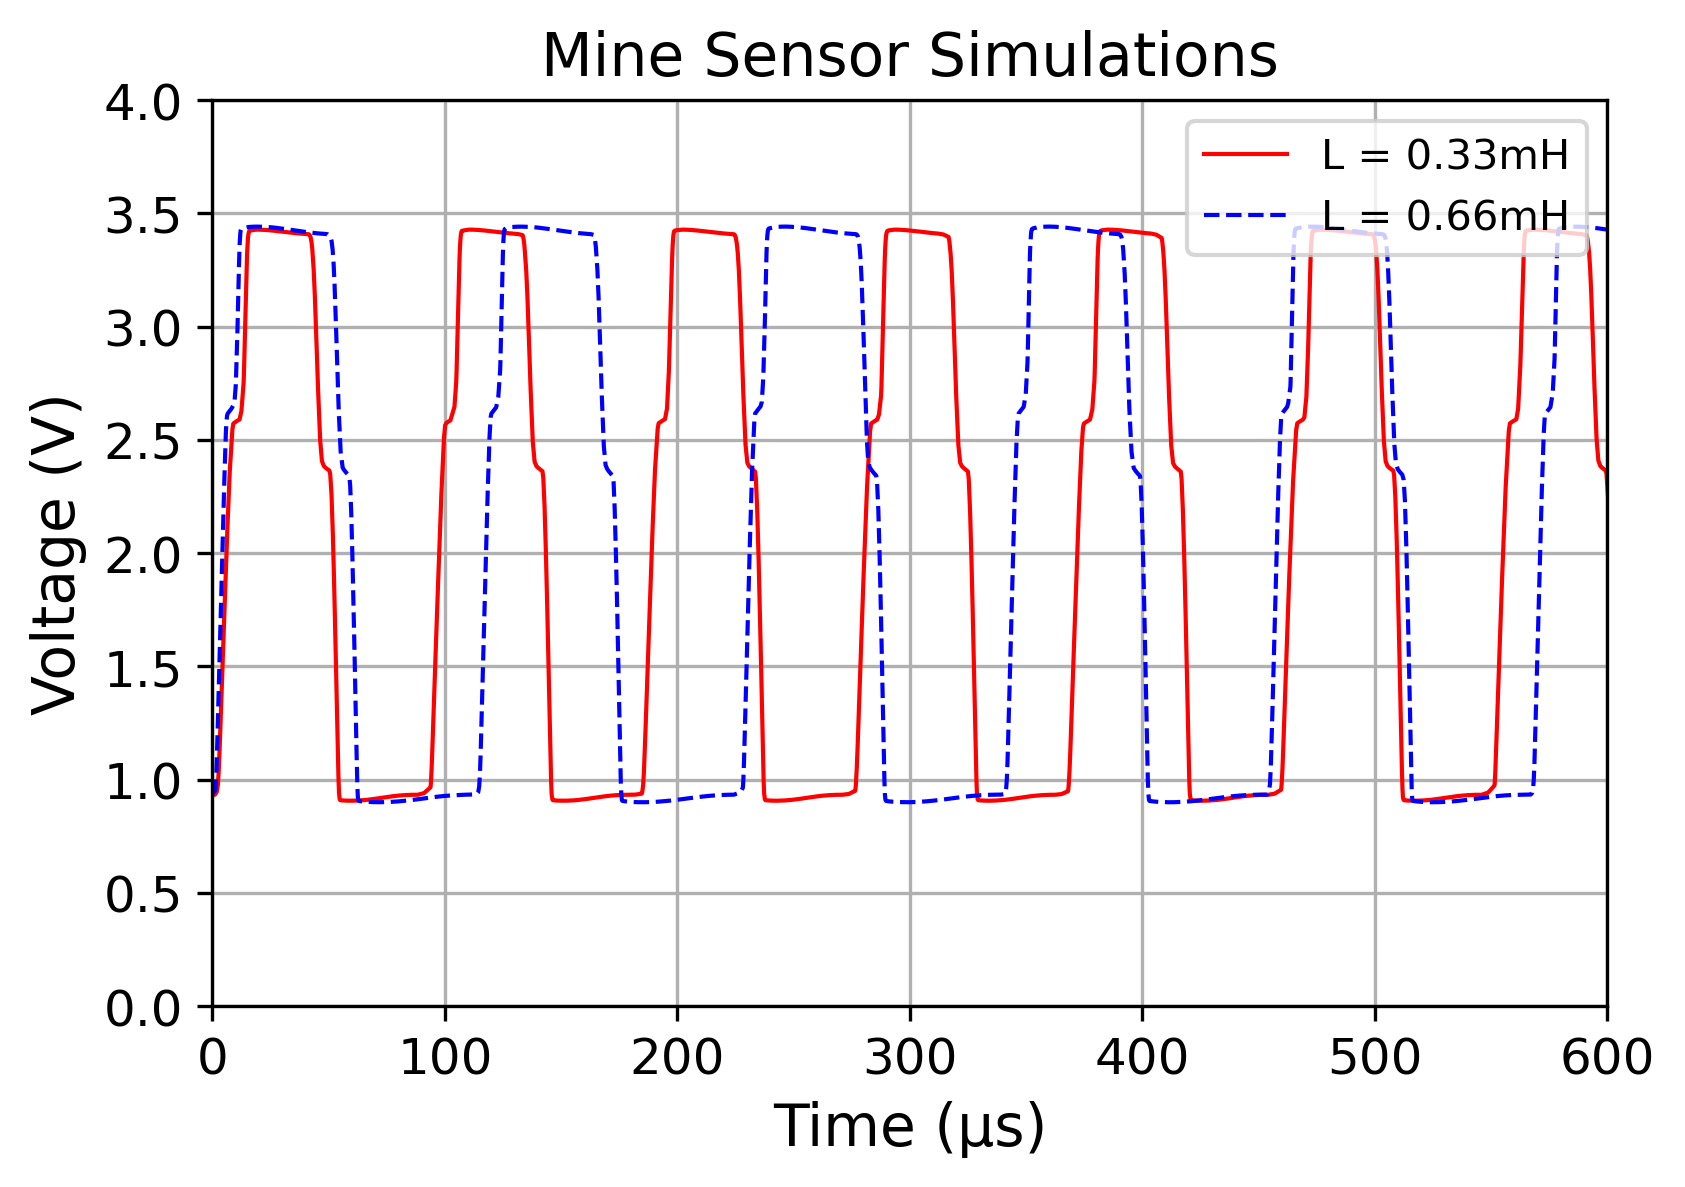
\includegraphics[scale = 0.7]{EPO 2 Images & Plots/Mine Sensor/666uH.png}
    \caption{Circuit Simulations}
    \label{fig:sim_sensor_neutral}
\end{figure}

Results of the simulations have shown the output of the circuit is indeed a square wave and the frequency of this square wave changes with an changing inductance value. In this case with an doubled inductance value from \(L=0.33mH\) to \(L = 0.66mH\) it is clearly shown in figure \ref{fig:sim_sensor_neutral} that the frequency of the square waves changes. An behaviour that should be expected. In the presence of the metal plate the inductance of the inductor increases giving a bigger period for the square wave. In reality the increase of inductance in presence of the 'mine' is around +10\%, this was measured using the XXX. %What was that decive called where you can measure all those components, inductance, capacitance and resistance.
In this simulation \(L=0.36mH\) is not given in the graph since the change in frequency is small and hardly noticeable in a graph. Nevertheless it doesn't matter that this value is not simulated since the main behaviour of; a changing period in presence of a changing inductance can also be simulated using \(L= 0.66mH\).\\
To sum up, the simulated output has a square wave function which period changes with a changing inductance. The simulated circuit works as expected.

\newpage
\section{Implementation}
\subsection{idk more things}
\\

\subsection{Code}
%Most likely this text has to be cut alot. To a more compact summary of the code.
After the sensor has been designed and simulated it will be built and integrated with the robot.
However, simply connecting the output of the sensor to the FPGA board is not yet enough. The output of this sensor still has to be processed to determine if a mine is detected or not.\\
With the use of some VHDL code the square wave output can be processed into determining whenever there is a mine detected or not.
As can be seen in the simulations, figure \ref{fig:sim_sensor_neutral}, the output of the sensor is a square wave functions. Which essentially has a high voltage and a low voltage, which the FPGA board reads as a '1' for high and '0' for low.\\
Since the '1' and '0' keeps its value for a few microseconds. We can count the amount of ones or zeros in 1 period. In presence of a metal mine, the inductance increases and thus also the period increases, which means the time the '1' and '0' holds in a period increases. Essentially if we know how many ones or zeros fit in one period without a mine. We can compare that with the amount of ones or zeros in a period with a mine. \\

Therefore the implemented code has a counter which in this case counts the amounts of zeros. In reality it doesn't really matter if the ones or zeros are counted, since the change in count due to a mine is important. The code is implemented using a FSM. The code has 4 stages, a reset stage, a counting stage, an compare stage, and a output stage. In communication with the other EPO-2 groups the output stage, the stage, which sends a '0' or '1' as output signaling that a mine had been detected, keeps on being on this stage for 10 milliseconds %%idk exact value anymore
so besides the FSM there is also a time counter which sends a '1' to the FSM when it is in the output stage and 10 milliseconds has passed. Which results the FSM to go back into its first stage, essentially resetting itself to start counting and detecting mines again. In the compare state the amount of zeros counted in one period gets compared to a set threshold. If it exceeds the threshold an '1' as output gets given in the output stage to the rest of the system, signaling a mine has been detected. The threshold for the code will be determined in the testing phase.

In Appendix XXX a visual FSD can be found and in Appendix XXX the code is given.

\subsection{Physical Placement Sensor}


\newpage
\section{The testing phase}
\subsection{Physical circuit testing}
After assembling the sensor circuit, it first will be tested whenever the circuit output also gives a square wave output as seen in the simulations.

Using a probe connected to the output, the output gets measured.

\begin{figure}[h]
    \centering
    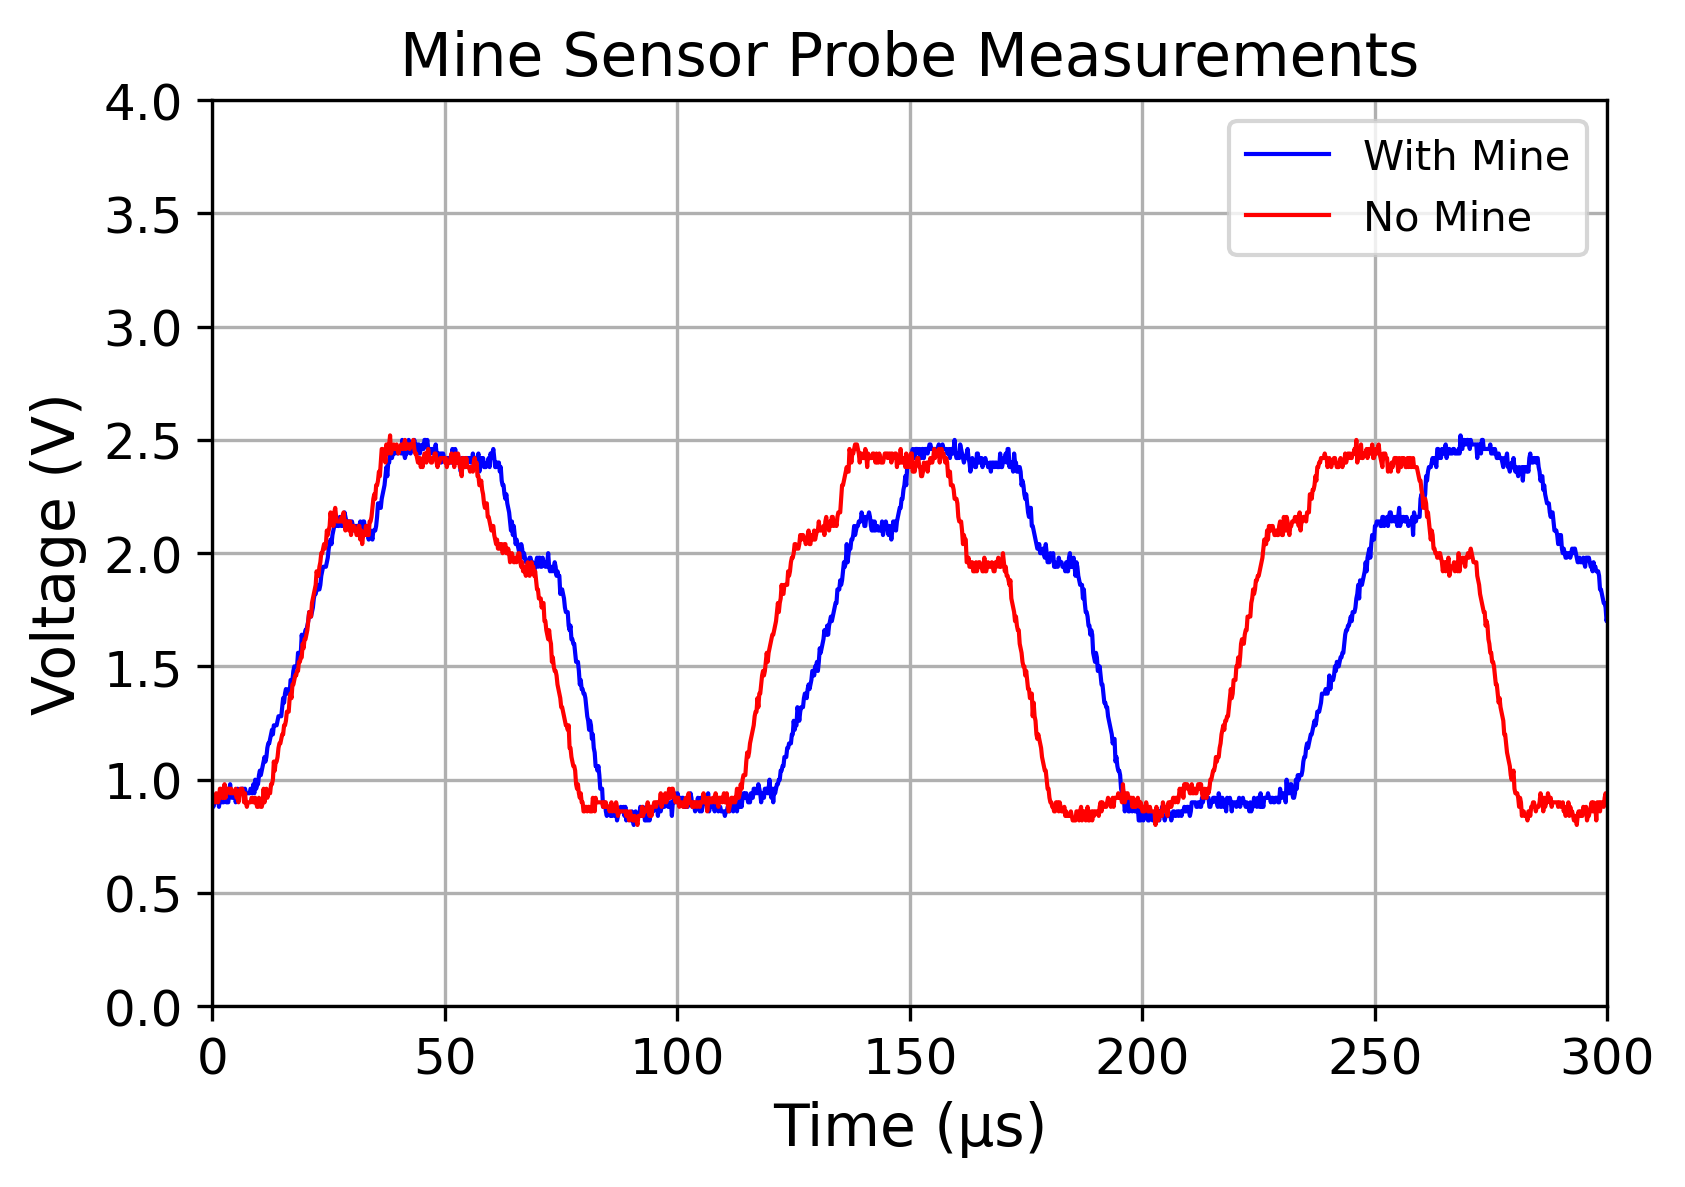
\includegraphics[scale = 0.7]{EPO 2 Images & Plots/Mine Sensor/V3_Total.png}
    \caption{Circuit Probe Measurements}
    \label{fig:meas_sensor_neutral}
\end{figure}

As seen in figure \ref{fig:meas_sensor_neutral} the output is mostly a square wave function. The FPGA board considers voltages above 1.2V as a '1'. So the two 'steps' are seen as a '1'. Essentially when looking carefully at the measurements, the amount of time that the signal is a '1' is longer than it is '0' in a period. This is not problematic since the change in the period under influence of a mine is important. So the shape of the 'square' wave signal is fine.\\
In figure \ref{fig:meas_sensor_neutral} the square wave is plotted with and without a mine. The graph shows a clear change in frequency and with a mine the period is bigger. Which is expected from the simulations. From this it can be concluded the sensor sufficiently senses the presence of a mine.\\
After testing the built circuit works as intended, the next step is to determine how many times '0' gets counted in 1 period. With this information a treshhold value can be set in the VHDL code.\\
The FPGA boards runs on a 50Mhz clock which has a 20 microseconds period. It must be determined how many of these 20 microseconds periods fit into the '0' state of the output square wave signal of 1 period. The time the signal is below the 1.2V could be measured with a oscilloscope. However the decision is made not to do this and instead to use the FPGA board directly to count the '0' state of the square wave. This is so that in the unlikely event that the circuit may behave a bit different on the FPGA board, the counted value is exactly is the actual value the FPGA board counts.
%%bla bla not yet finished.


\newpage
\subsection{Sensor FPGA board implementation testing}
A simple VHDL code which counts how many periods of 20 microseconds fit into the low state of the square wave for 1 period was written, with a bit vector as output. This output was displayed on the FPGA board using the leds. This gave 2112 counts without a mine and 2400 counts with a mine.
After further testing and testing with the actual VHDL sensor code with the different values as threshold. A final threshold value of 2350 counts was chosen.\\

After a threshold was chosen the sensor with VHDL code can be tested. After the VHDL Code was implemented on the FPGA board. Two states, the counting stage and the compare stated where checked if they work as intended. By designating a led to each state, a probe was connected to the led to see the states on the oscilloscope.

\begin{figure}[!h]
    \begin{minipage}{0.5\textwidth}
     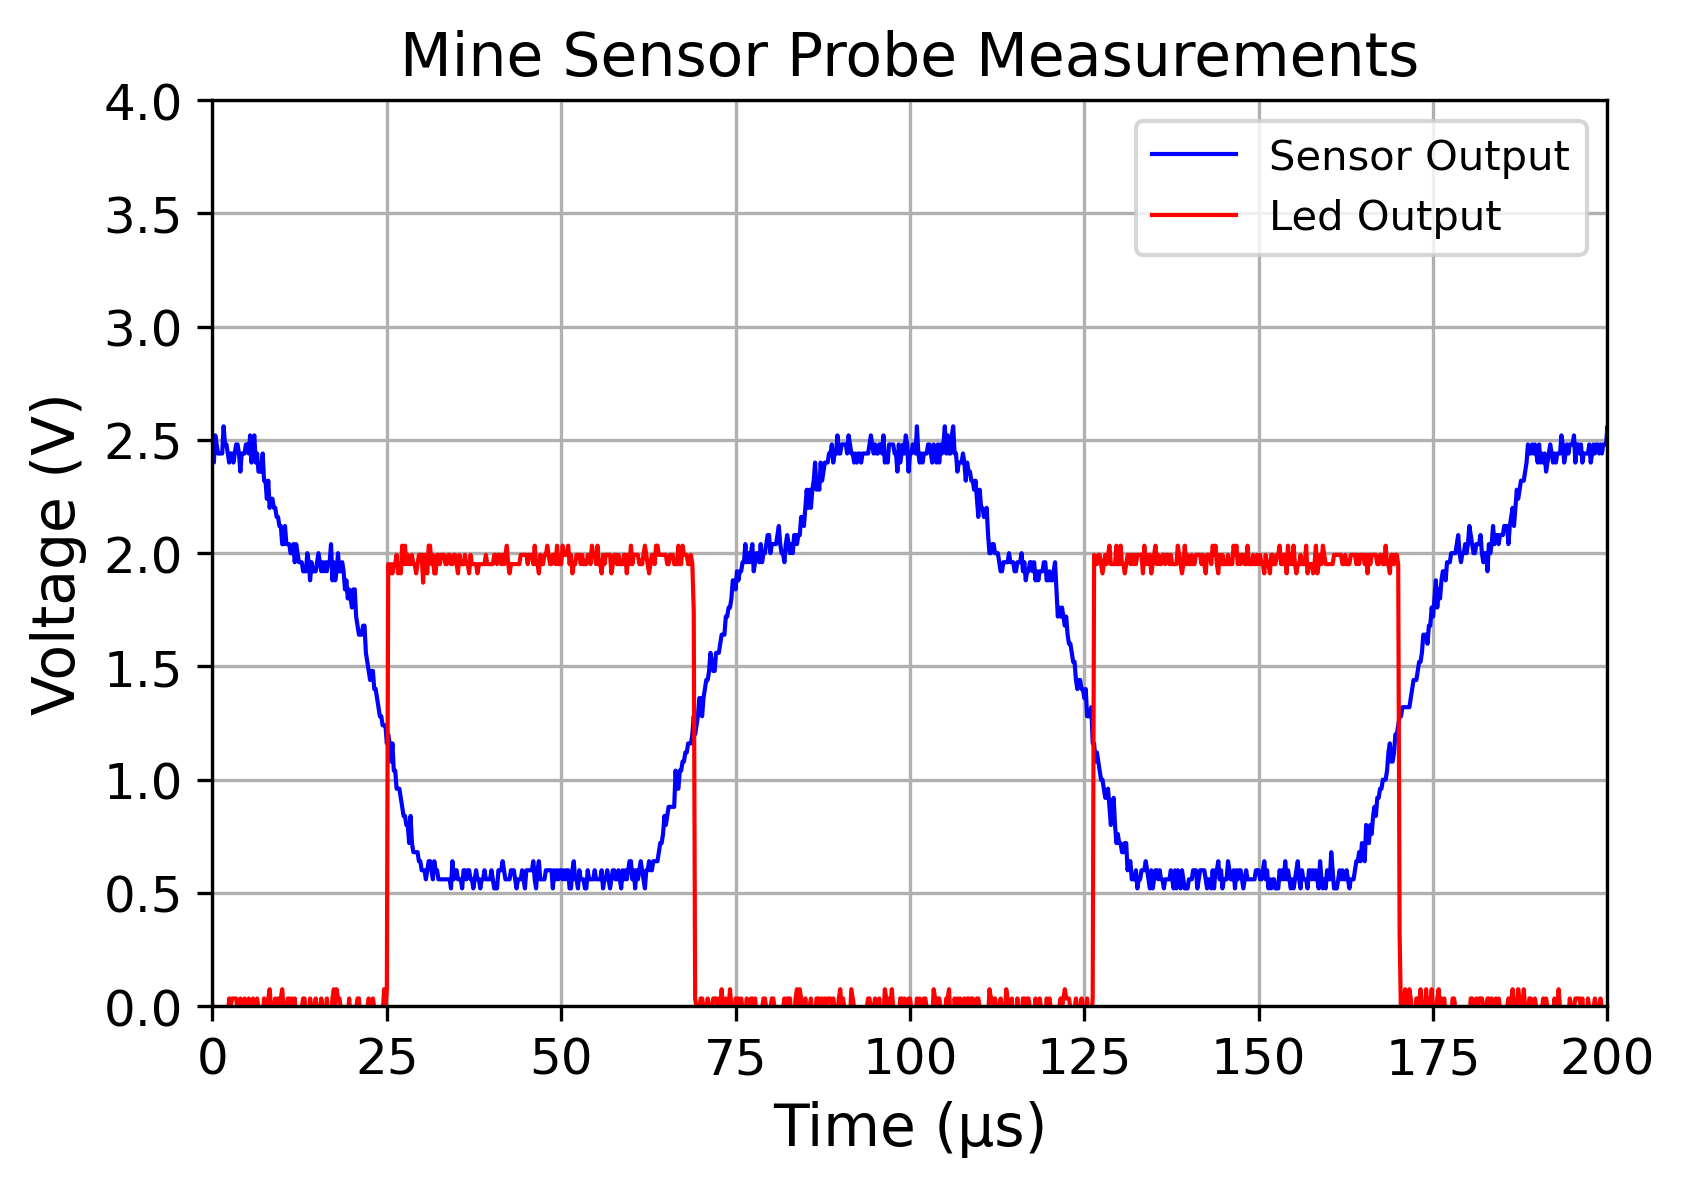
\includegraphics[width=\linewidth]{EPO 2 Images & Plots/Mine Sensor/V3_Count_Stage_No_Mine.png}
     \caption{Count state}
     \label{fig:meas_count}
    \end{minipage}
    \hfill
    \begin{minipage}{0.5\textwidth}
      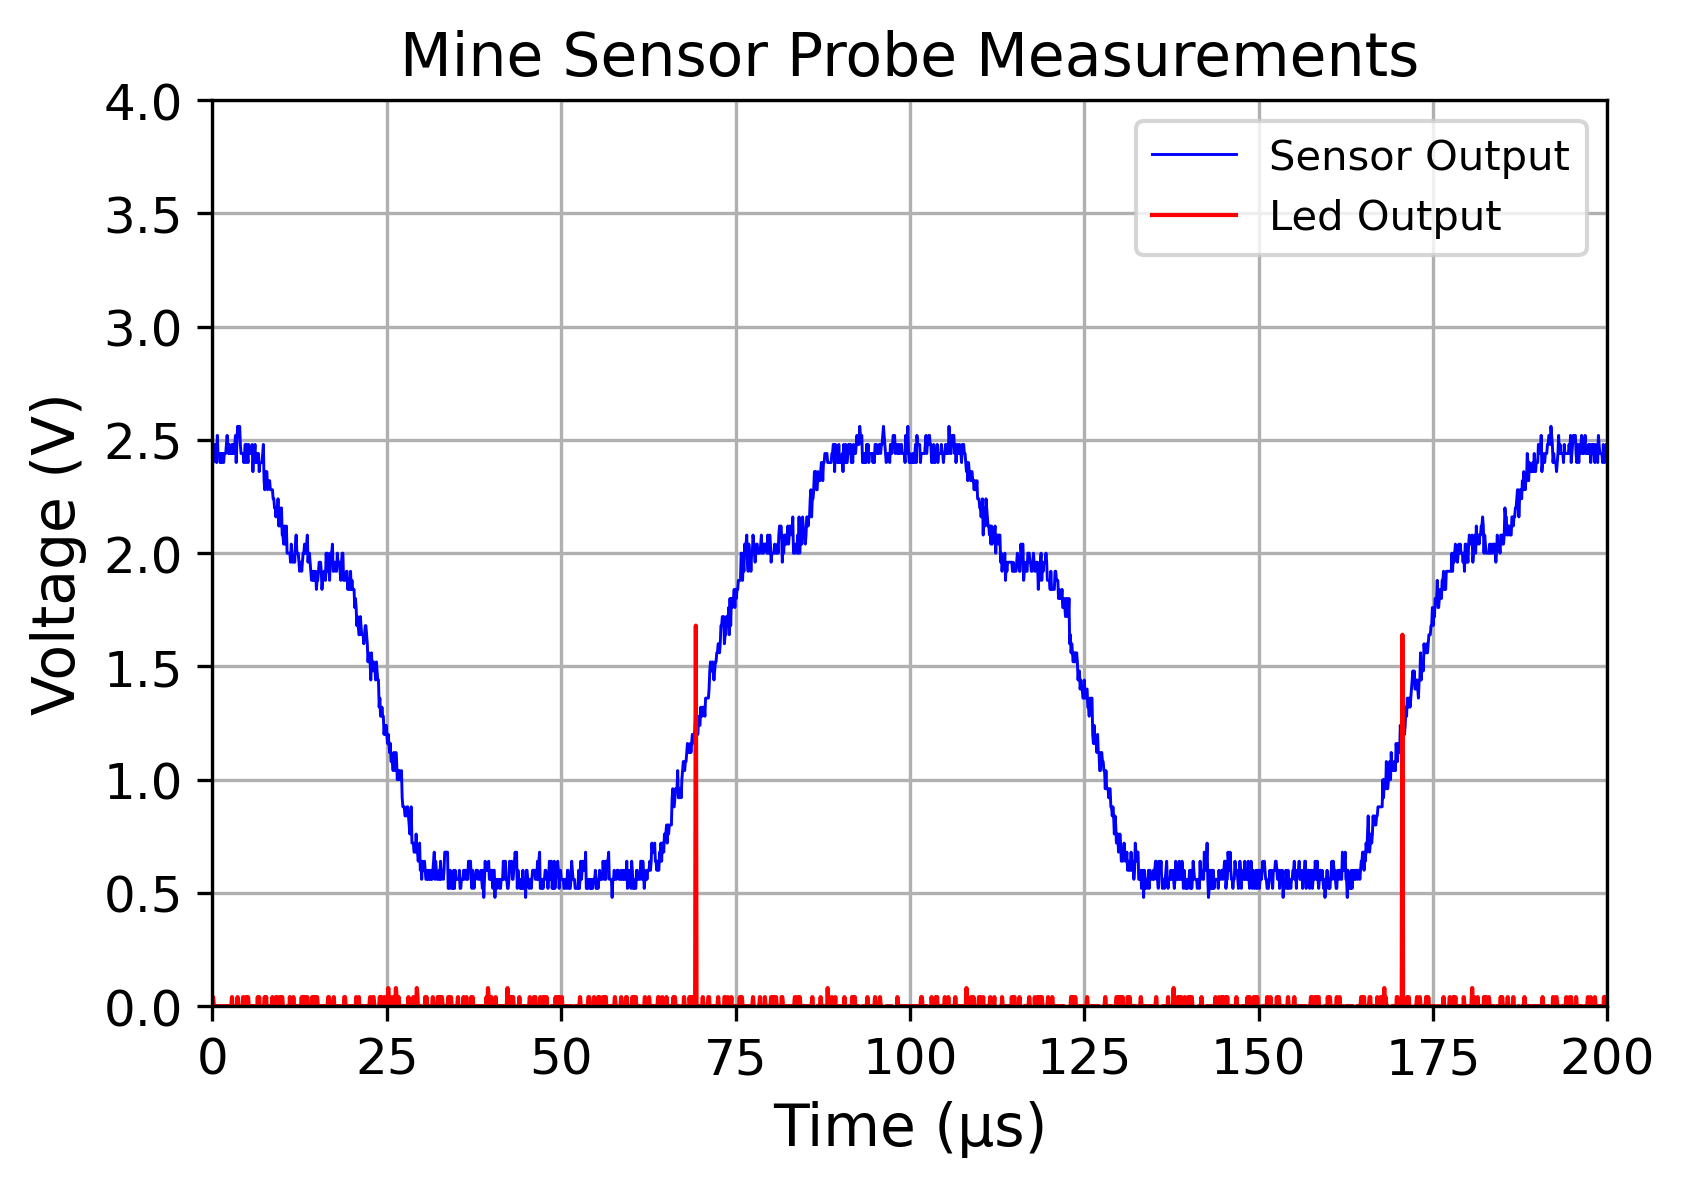
\includegraphics[width=\linewidth]{EPO 2 Images & Plots/Mine Sensor/V3_Compare_State_No_Mine.png}
      \caption{Compare state}
      \label{fig:meas_compare}
    \end{minipage}
\end{figure}

As can be seen in figures \ref{fig:meas_count} and \ref{fig:meas_compare} the counting state can be seen when the square wave signal is '0' and the compare state can be seen at the end of the '0' signal when the square wave jumps to a higher voltage. This shows us the VHDL Code is indeed counting when the square wave signal is low and after counting immediately goes to the compare state. Out of visual observations where the output in the output state is assigned to a LED. It could be seen that the LED lights up when an metal object is placed below it and stays off when there is nothing below the sensor. From these observations and measurements it can be said confidentially that the sensor and the code works as intended.

